\documentclass[UTF8,a4paper]{article}
\usepackage{fancyhdr}
\usepackage{ctex}
\usepackage{amsmath}
\usepackage{listings}
\usepackage{color}
\usepackage{graphics}
\usepackage{graphicx}
\lstset{ %
	extendedchars=false,            % Shutdown no-ASCII compatible
	language=Matlab,                % choose the language of the code
	basicstyle=\small\sf,    % the size of the fonts that are used for the code
	tabsize=3,                            % sets default tabsize to 3 spaces
	numbers=left,                   % where to put the line-numbers
	numberstyle=\tiny,              % the size of the fonts that are used for the line-numbers
	stepnumber=1,                   % the step between two line-numbers. If it's 1 each line
	% will be numbered
	numbersep=5pt,                  % how far the line-numbers are from the code   %
	keywordstyle=\color[RGB]{33,33,234},               % keywords
	commentstyle=\color[RGB]{0,0,0},    % comments
	stringstyle=\color[rgb]{0.170,0.187,0.102},      % strings
	backgroundcolor=\color{white}, % choose the background color. You must add \usepackage{color}
	showspaces=false,               % show spaces adding particular underscores
	showstringspaces=false,         % underline spaces within strings
	showtabs=false,                 % show tabs within strings adding particular underscores                frame = single,         % adds a frame around the code
	captionpos=b,                   % sets the caption-position to bottom
	breaklines=true,                % sets automatic line breaking
	breakatwhitespace=false,        % sets if automatic breaks should only happen at whitespace
	title=\lstname,                 % show the filename of files included with \lstinputlisting;
	% also try caption instead of title
	mathescape=true,escapechar=?    % escape to latex with ?..?
	escapeinside={\%*}{*)},         % if you want to add a comment within your code
	%columns=fixed,                  % nice spacing
	%morestring=[m]',                % strings
	%morekeywords={%,...},%          % if you want to add more keywords to the set
	%    break,case,catch,continue,elseif,else,end,for,function,global,%
	%    if,otherwise,persistent,return,switch,try,while,...},%
}
\pagestyle{fancy}
\lhead{}
\chead{}
\rhead{\bfseries The Matlab $6^{th}$ Homework}
\lfoot{}
\cfoot{\thepage}
\rfoot{}
\renewcommand{\headrulewidth}{0.4pt}
\begin{document}
\begin{center}
    \textbf{\LARGE{Matlab $6^{th}$ Homework}}\\[0.5cm]
    \normalsize{庄震丰 22920182204393}\\[0.5cm]
    \large{NOV. $7^{th}$, 2019}
\end{center}
\section{Limit}
\subsection{Plot Signal Curves}
 
$$
\begin{aligned}
    &(2-e^(-t))u(t)\\
    &t[u(t)-u(t-1)]\\
    &[1+cos(\pi t)][u(t)-u(t-2)]\\
    &u(cos(t))
\end{aligned}
$$
\subsection{Analysis}
\noindent To generate step function u(t),use \textbf{stepfun()} or \textbf{heaviside()}.
\subsection{Codes and Result}
\textbf{Question 1}
\begin{lstlisting}
    ezplot('(2-exp(-t)).*stepfun(t,0)',[-3,3]);
\end{lstlisting}
\textbf{Result}\\
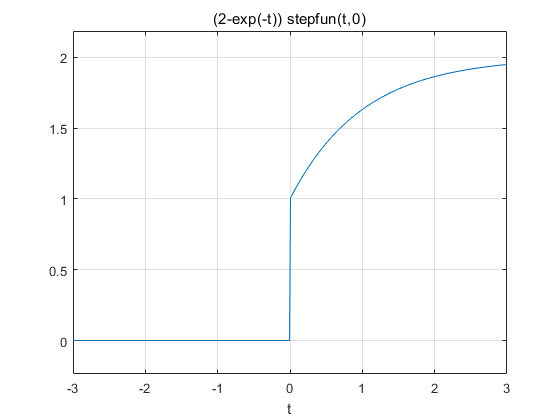
\includegraphics[scale=0.6]{1-1.png}\\
\textbf{Question 2}\\
\begin{lstlisting}
    ezplot('t.*(stepfun(t,0)-stepfun(t,1))',[-3,3]);
\end{lstlisting}
\textbf{Result}\\
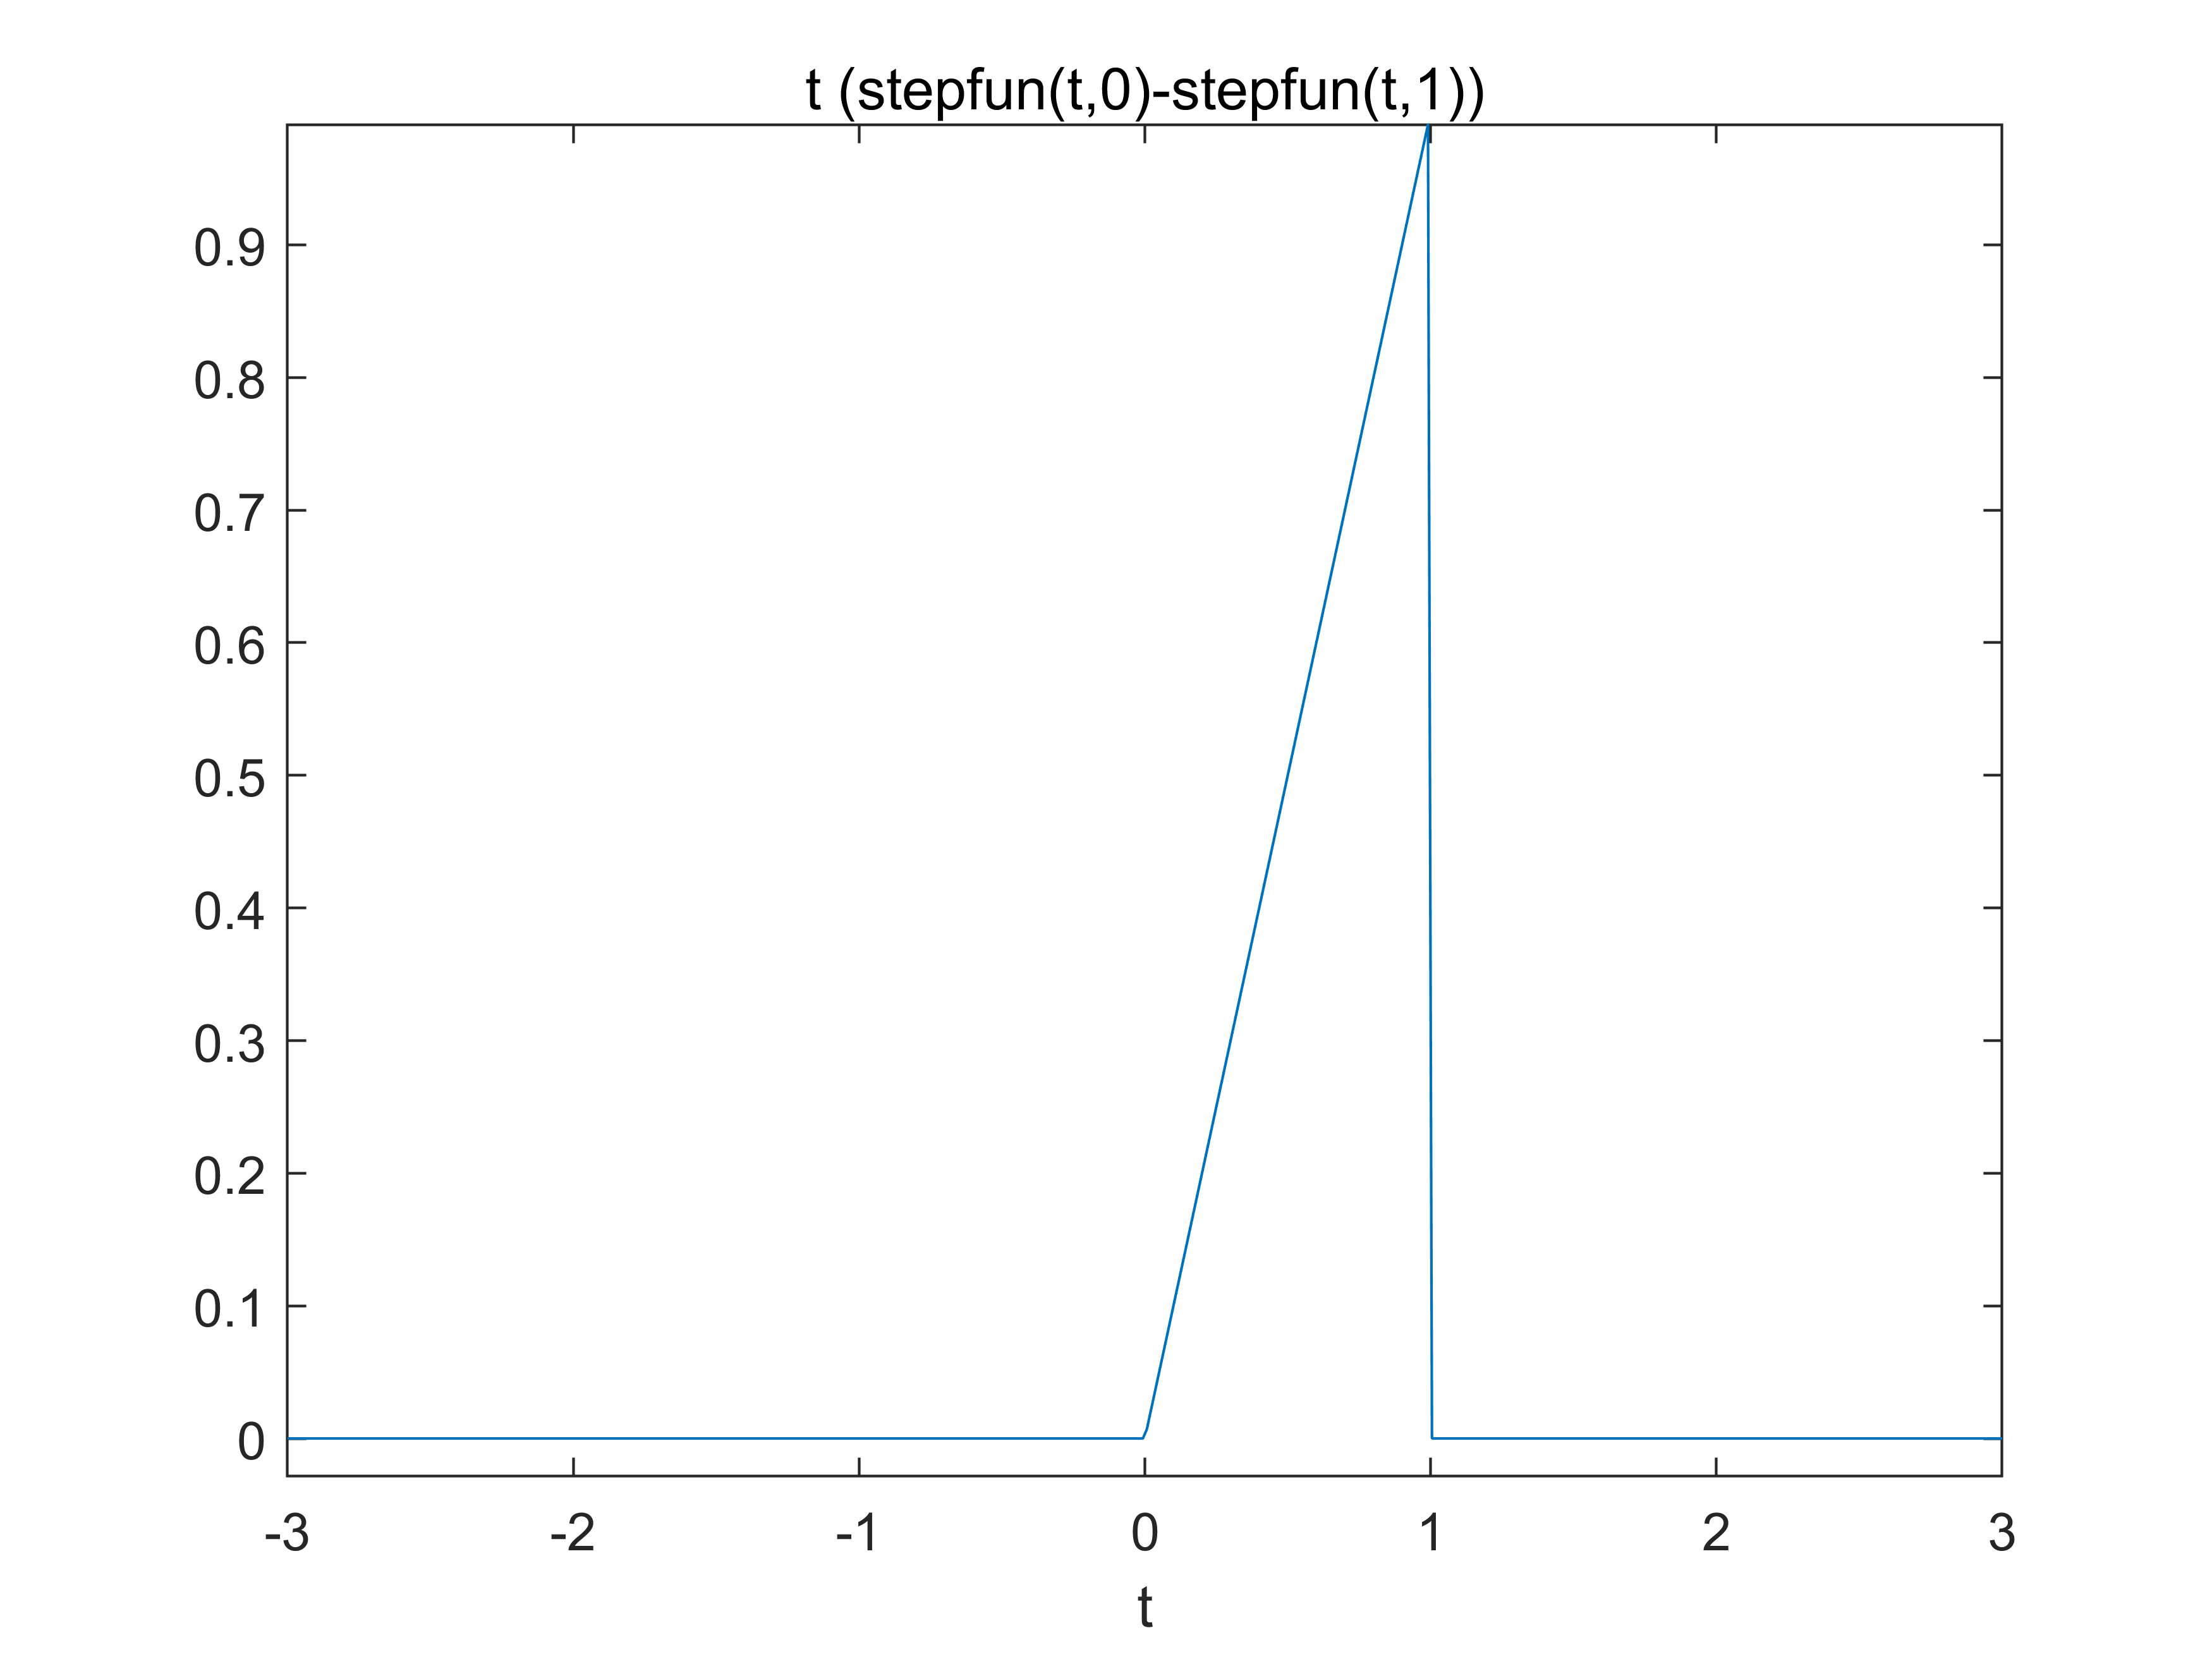
\includegraphics[scale=0.6]{1-2.png}\\
\textbf{Question 3}
\begin{lstlisting}
ezplot('(stepfun(t,0)-stepfun(t,2)).*(1+cos(pi*t))',[-3,3]);
grid on;
title('$(1+cos(\pi t))(u(t)-u(t-2))$','Interpreter','Latex');  
\end{lstlisting}
\textbf{Result}\\
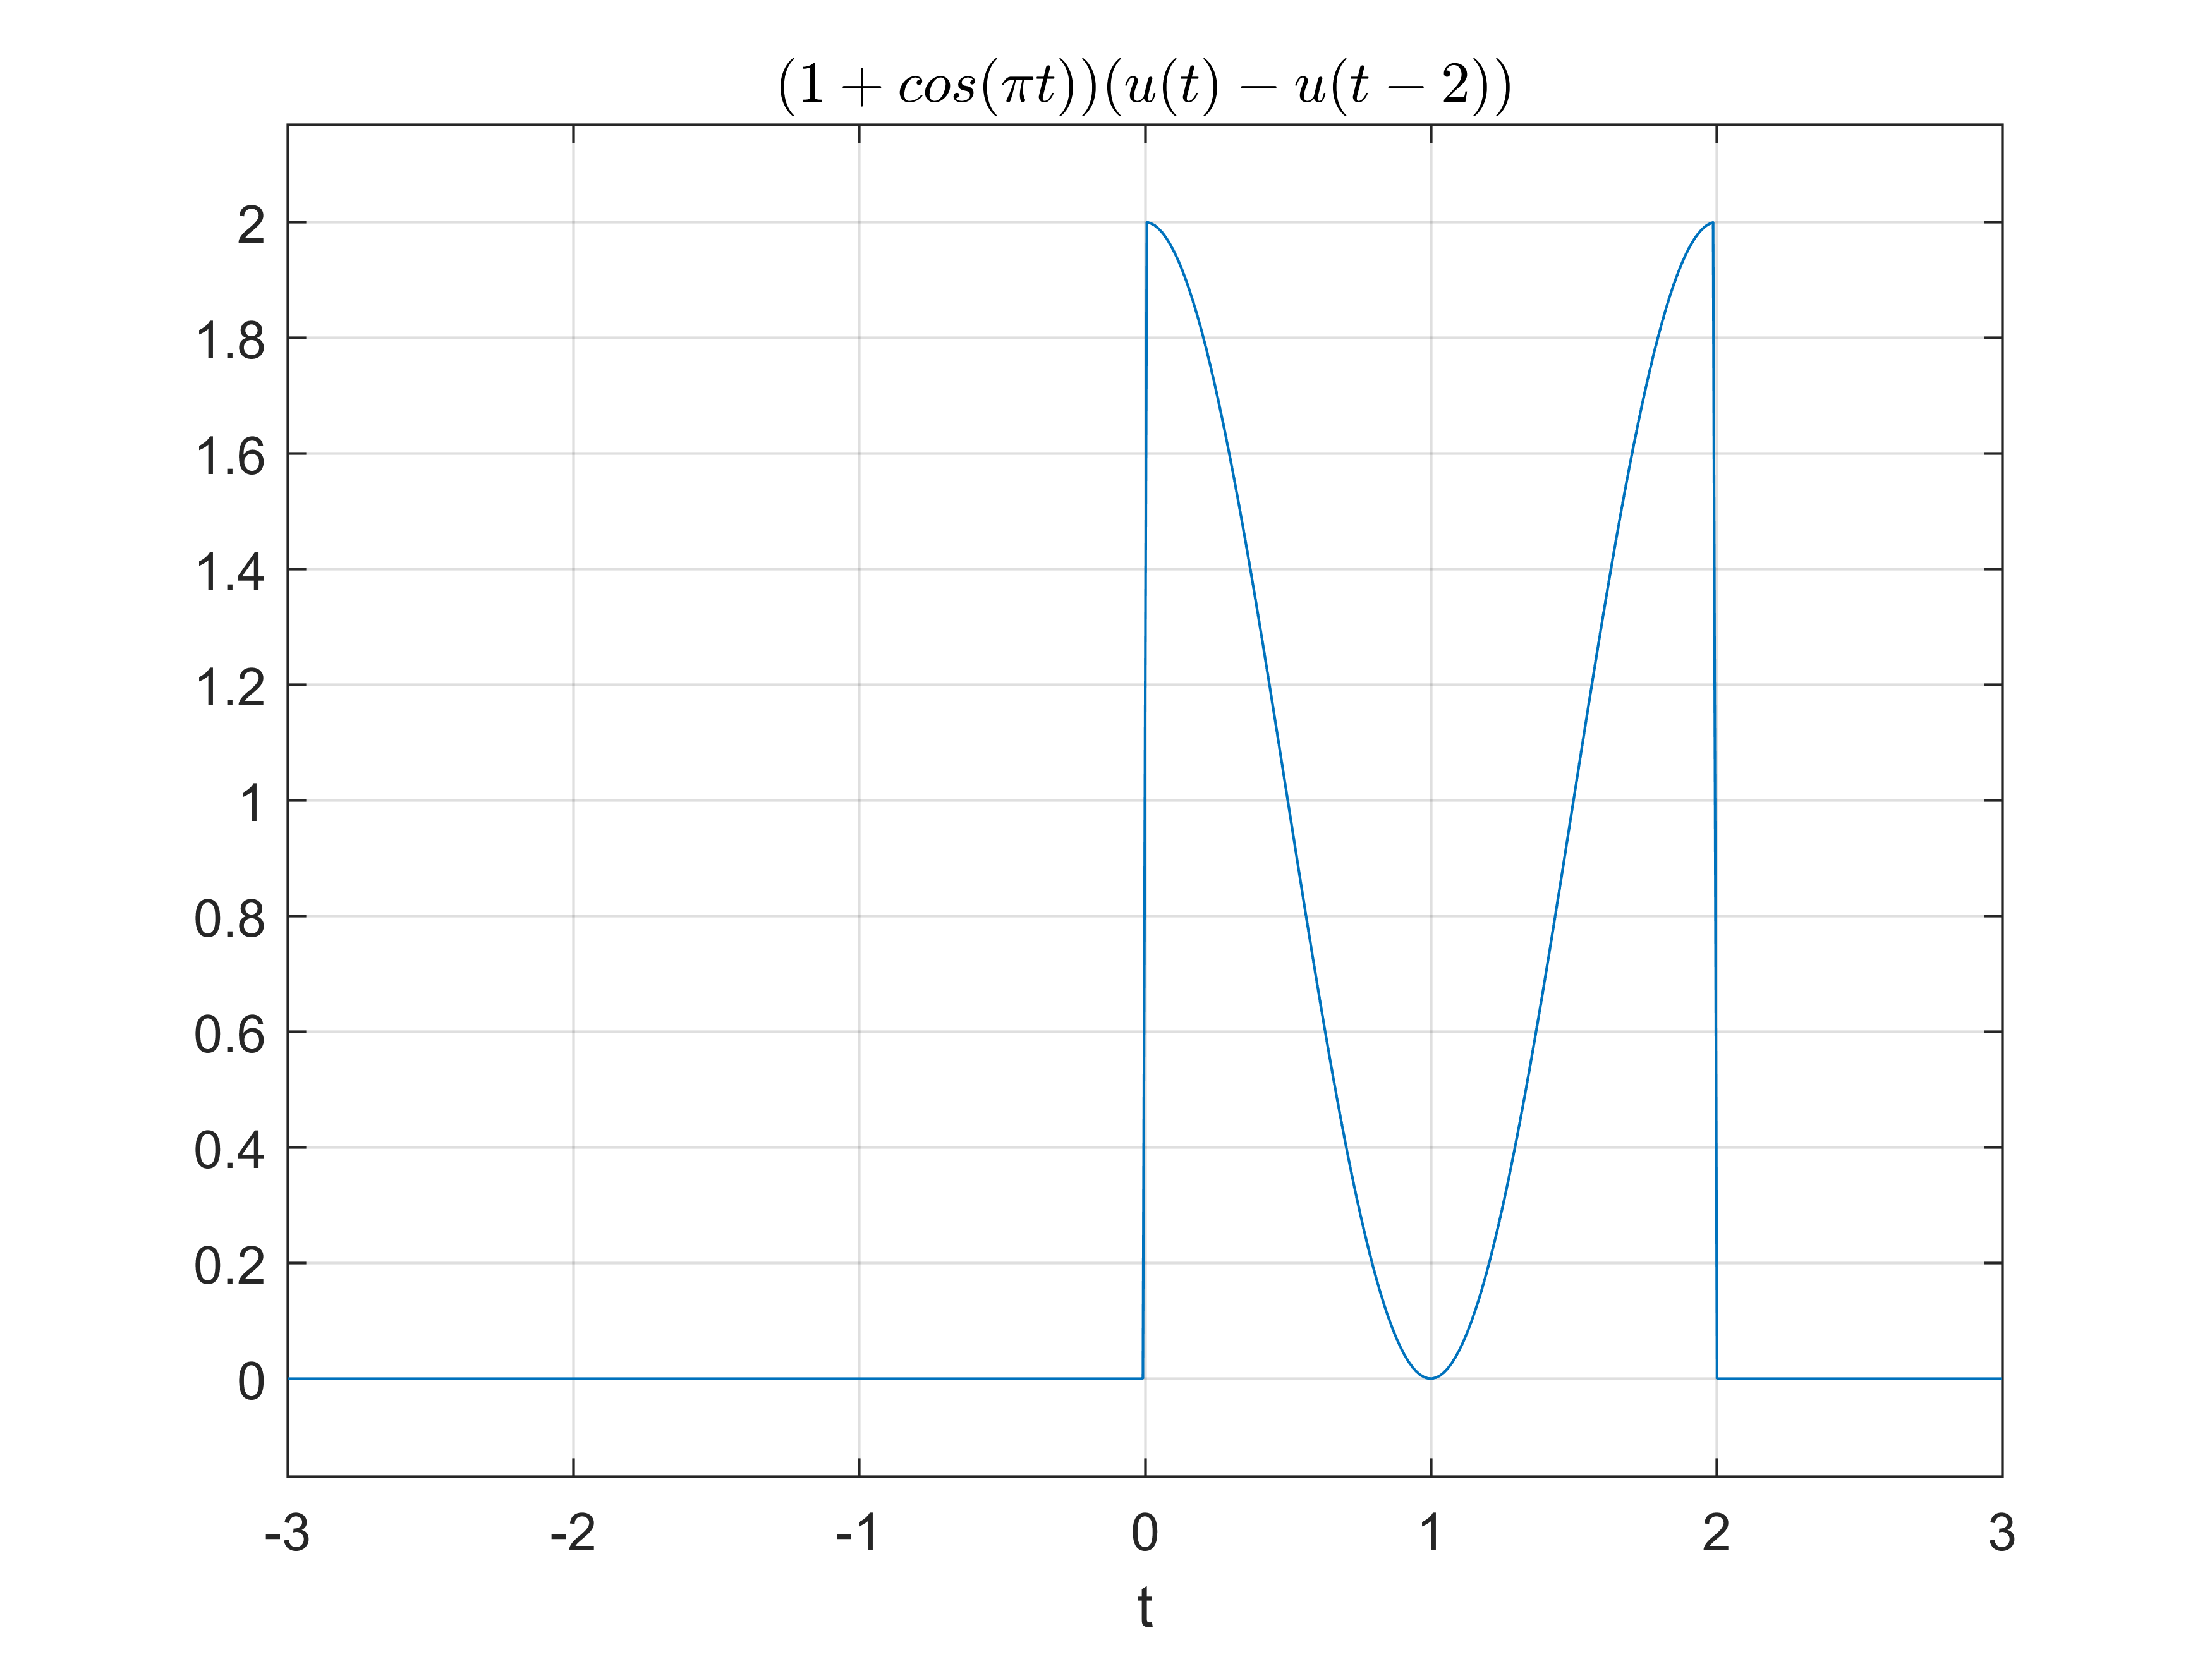
\includegraphics[scale=0.65]{1-.png}\\
\textbf{Question 4}\\
\begin{lstlisting}
    t=-10:0.01:10;
    y=heaviside(cos(t));
    plot(t,y)
    grid on;
    hold on;
    title('u(cos(t))');
    xlabel('t');
    ylabel('y')
\end{lstlisting}
\textbf{Result}\\
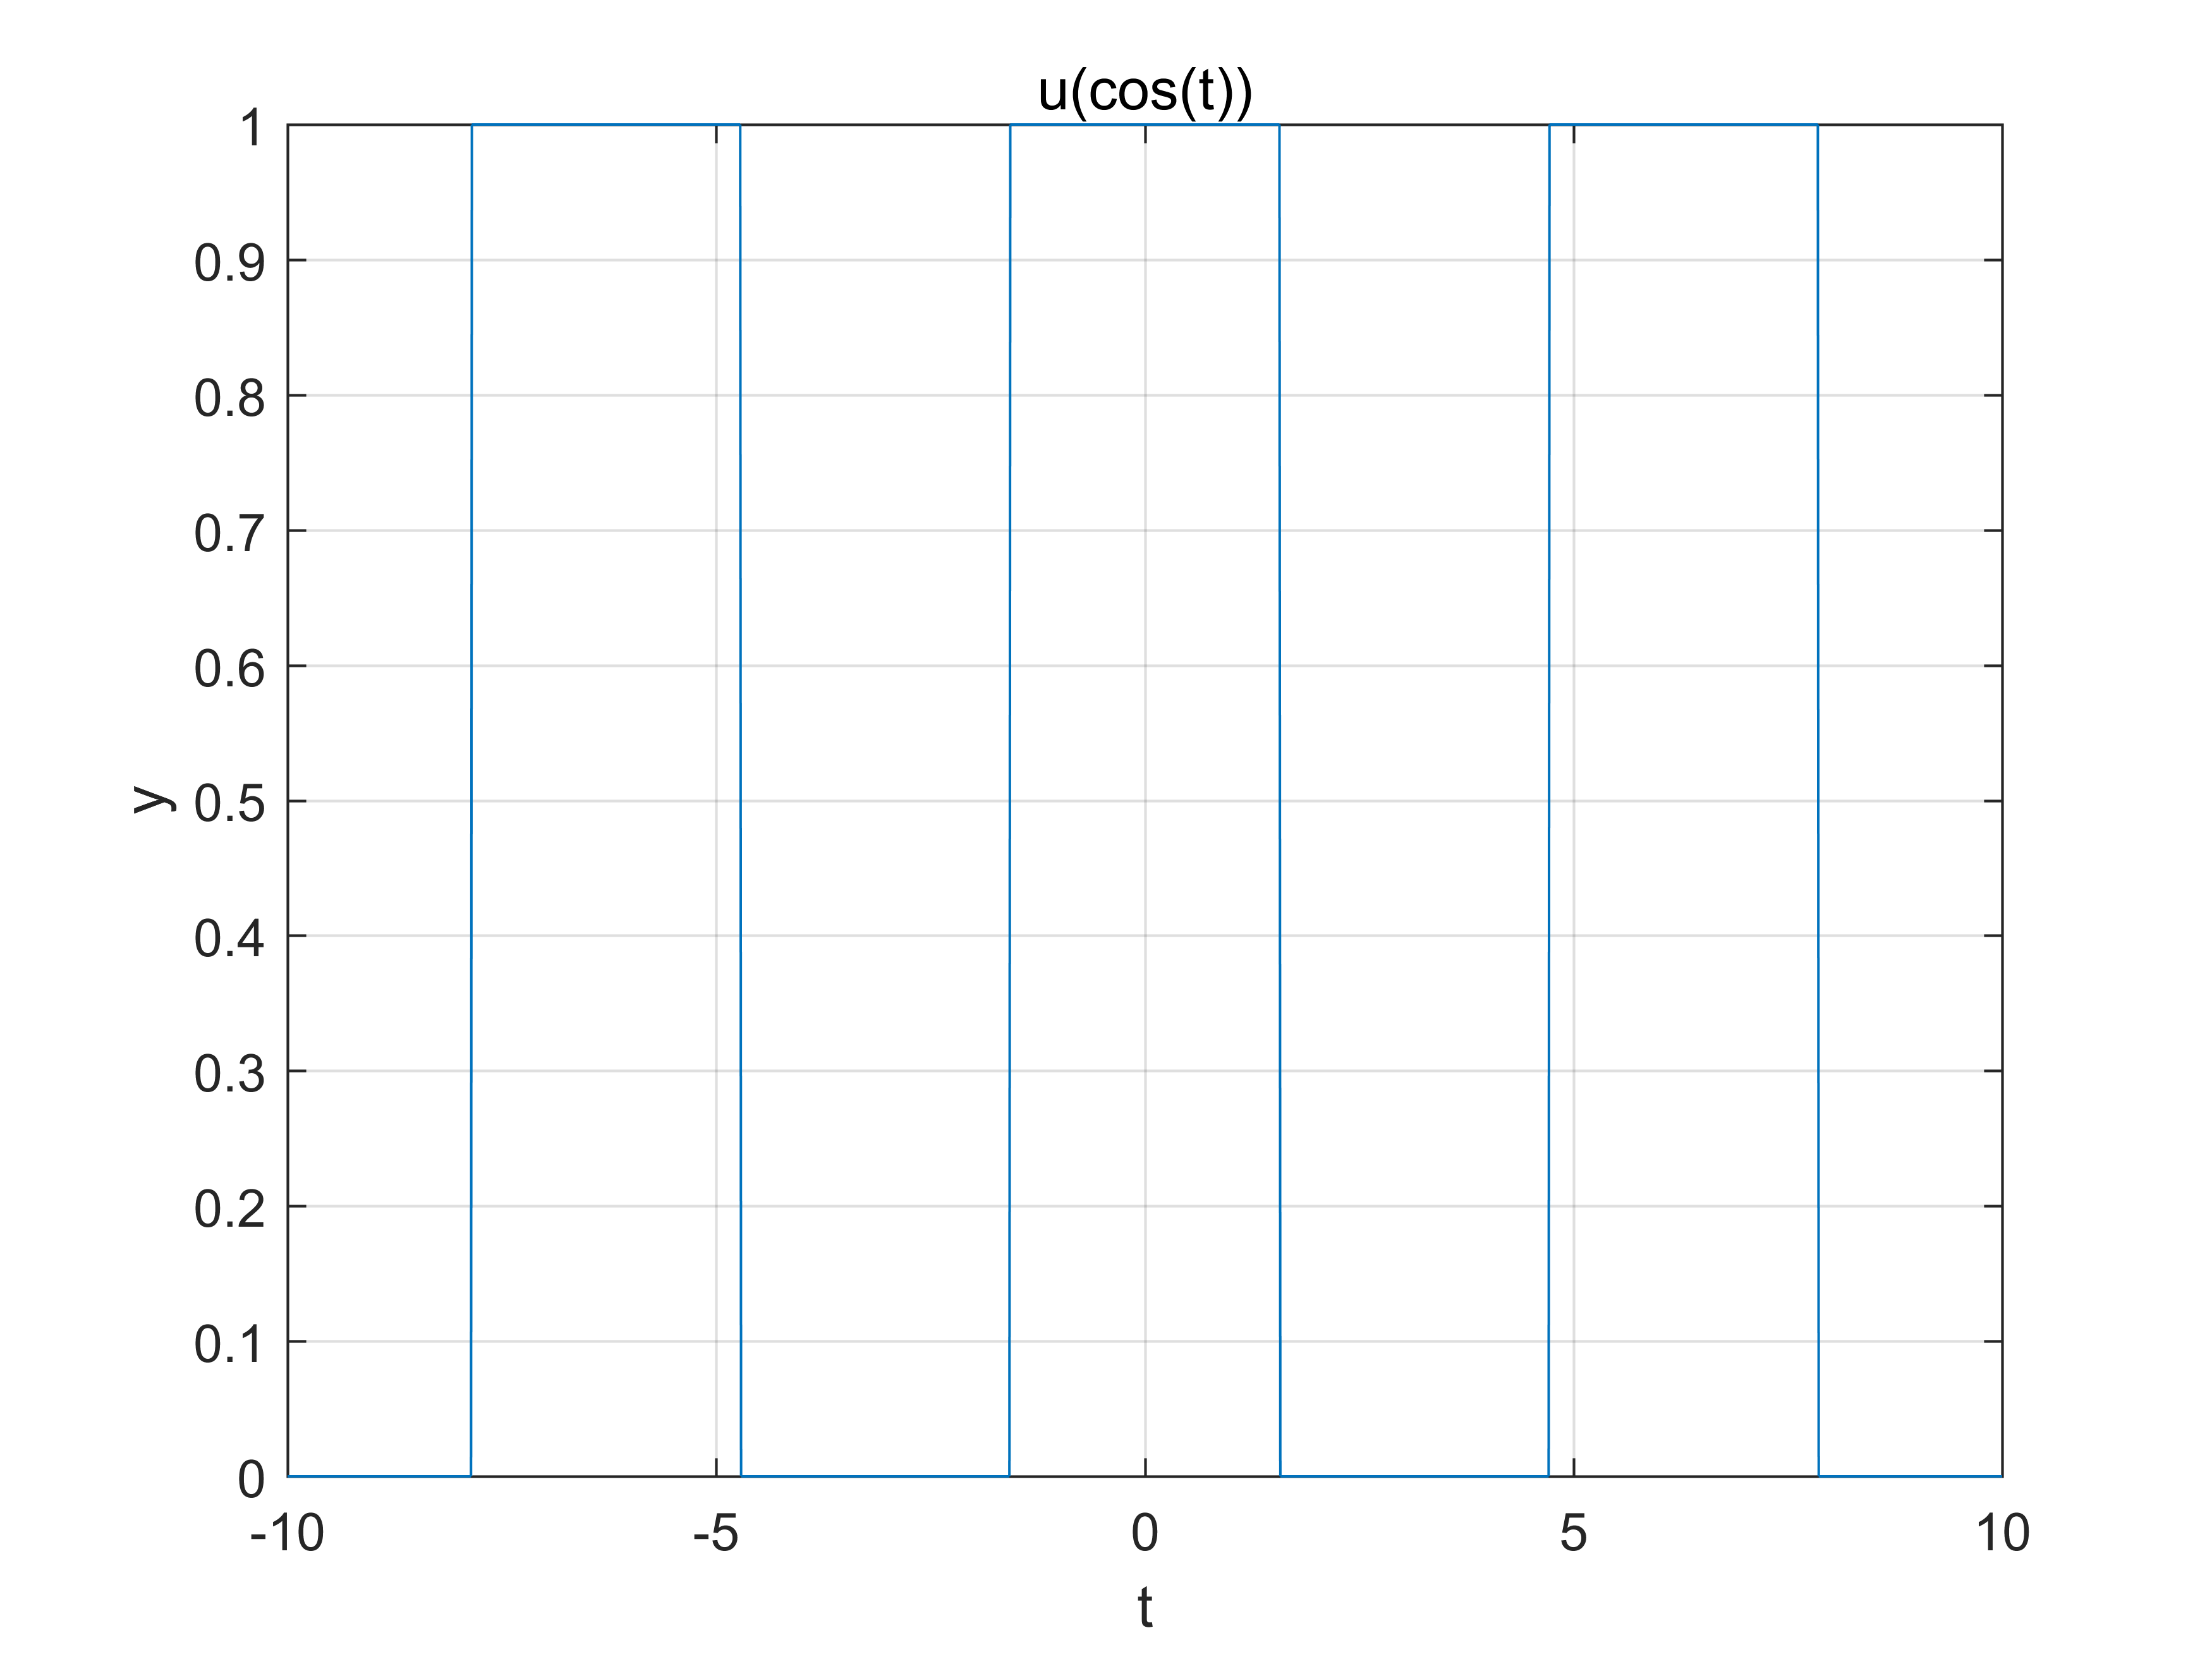
\includegraphics[scale=0.6]{1-4.png}\\

\section{complex Plot}
\subsection{Description}
Draw the real, imaginary, mold, and spoke angle of the following complex signals.
\begin{center}
$f(t)=2+e^{j\frac{\pi}{4}t}+e^{j\frac{\pi}{2}t}$
\end{center}
\subsection{Anaylsis}
\noindent use function \textbf{real(),imag(),angle(),abs()}.
\subsection{Code and Result}
\begin{lstlisting}
t=-3:0.01:3;
f=2+exp(j*pi/4*t)+exp(j*pi/2*t);
subplot(2,2,1);
plot(t,real(f));title('real');grid on;
subplot(2,2,2);
plot(t,imag(f));title('imag');grid on;
subplot(2,2,3);
plot(t,abs(f));title('abs');grid on;
subplot(2,2,4);
plot(t,angle(f));title('angle');grid on;           
\end{lstlisting}
\textbf{Result}\\
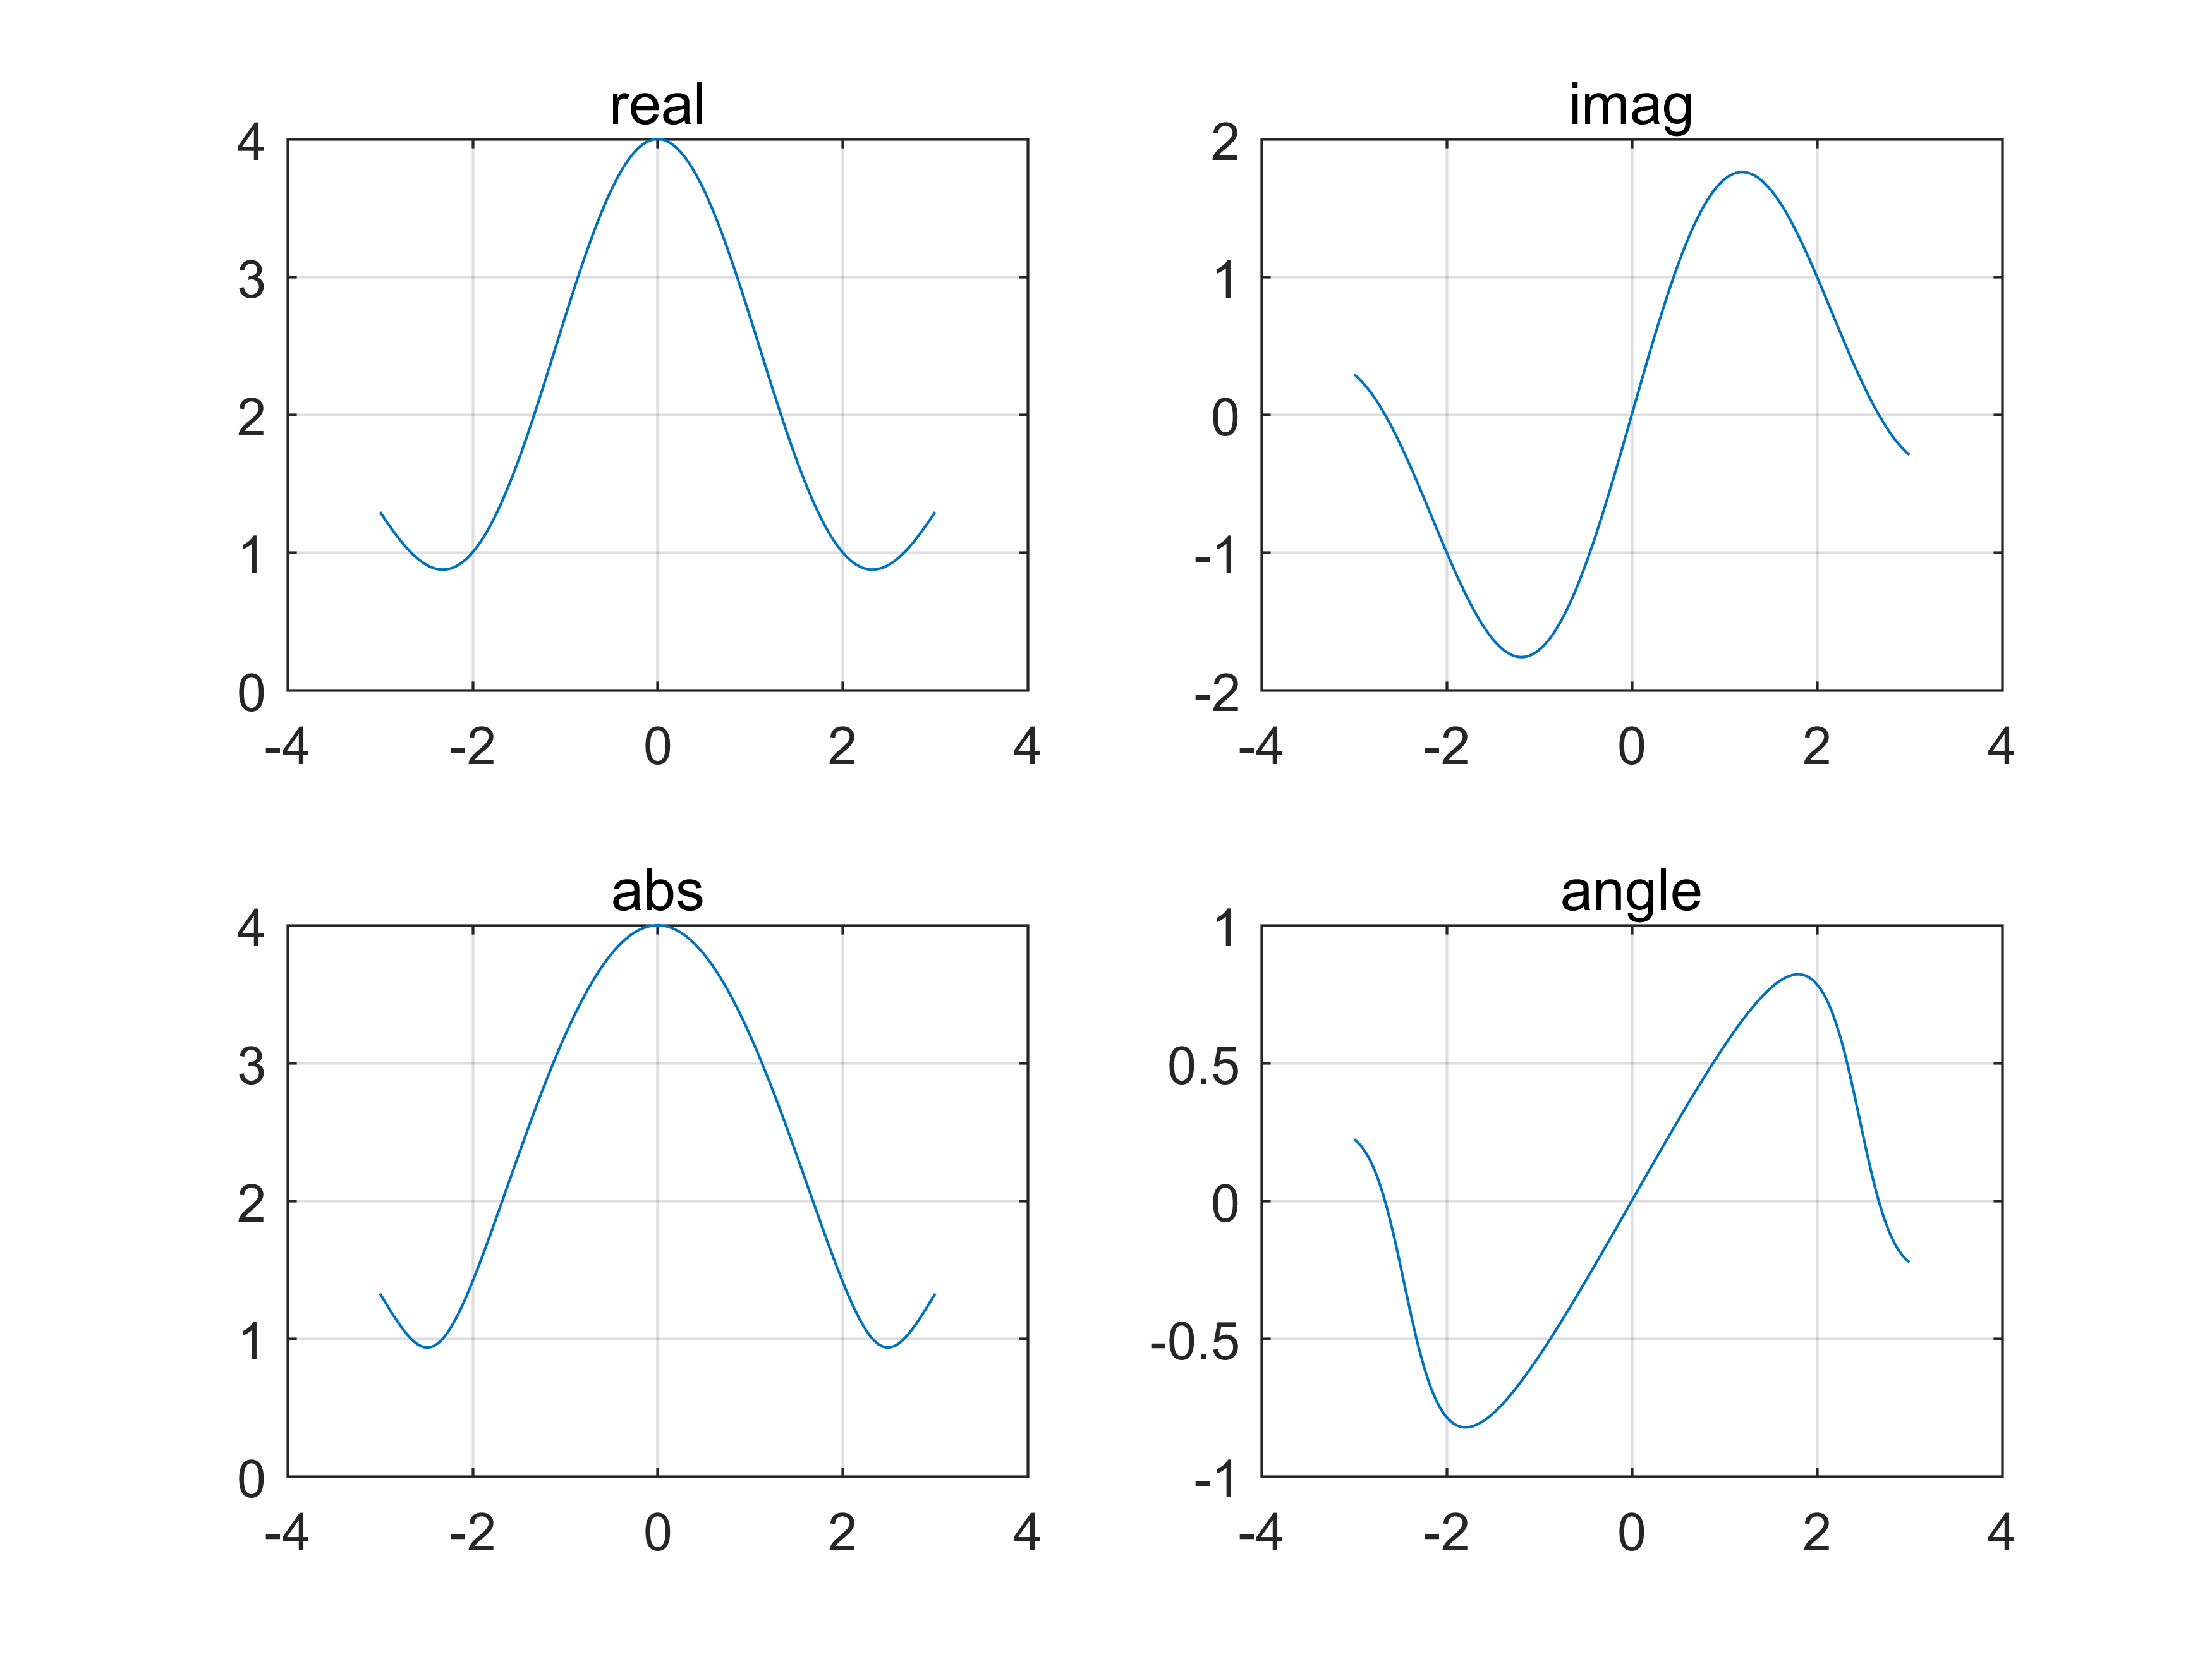
\includegraphics[scale=0.7]{2.png}\\

\section{Rectangular pulse signal}
\subsection{Description}
Produce a cycle rectangular pulse signal with a amplitude of 1, a period of 1, and a duty cycle of 0.5
\subsection{Anaylsis}
\noindent Use function \textbf{square(2*pi*T,duty)}
\subsection{Code and Result}
\begin{lstlisting}
    t=-4:0.01:4;
    y=square(2*pi*t,50);
    plot(t,y);
    hold on;
    grid on;
    title('square');
    xlabel('t');
    ylabel('square');
    axis([-4,4,-1.1,1.1]);
\end{lstlisting}
\textbf{Result}\\
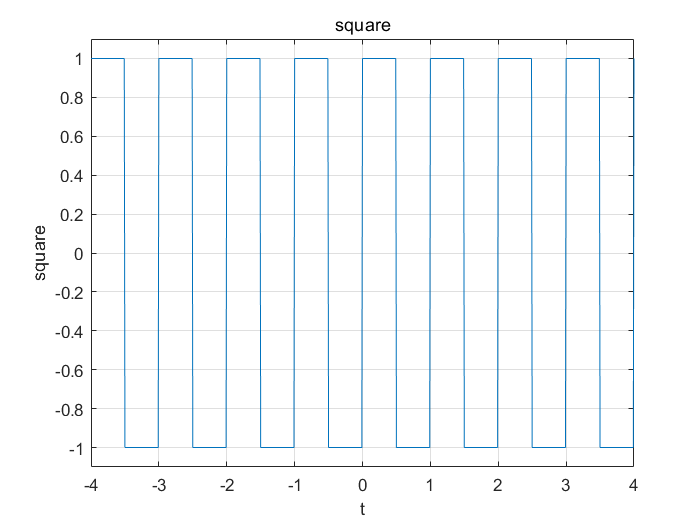
\includegraphics[scale=0.6]{3.png}\\

\section{Plot signal f}
\subsection{Description}
Plot $f(t)=\frac{sin \pi t}{t}$ and f(2t) f(1-0.5t).
\subsection{Anaylsis}
\noindent Use \textbf{ezplot(),sinc(T*2*$\pi$)}. 
\subsection{Code and Result}
\begin{lstlisting}
    syms t
    f=sinc(t)*pi;
    ezplot(f);
    hold on;
    ezplot(subs(f,t,2*t));
    ezplot(subs(f,t,1-0.5*t));
    grid on;
    legend('f','f(2t)','f(1-0.5t)')
\end{lstlisting}
\textbf{Result}\\
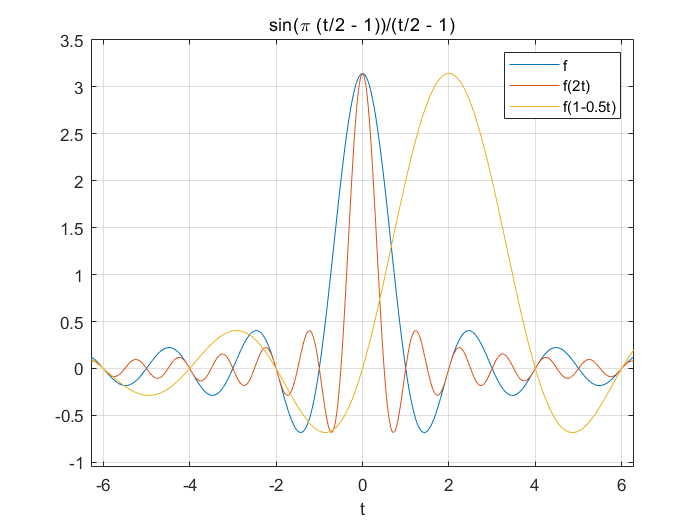
\includegraphics[scale=0.6]{4.png}\\
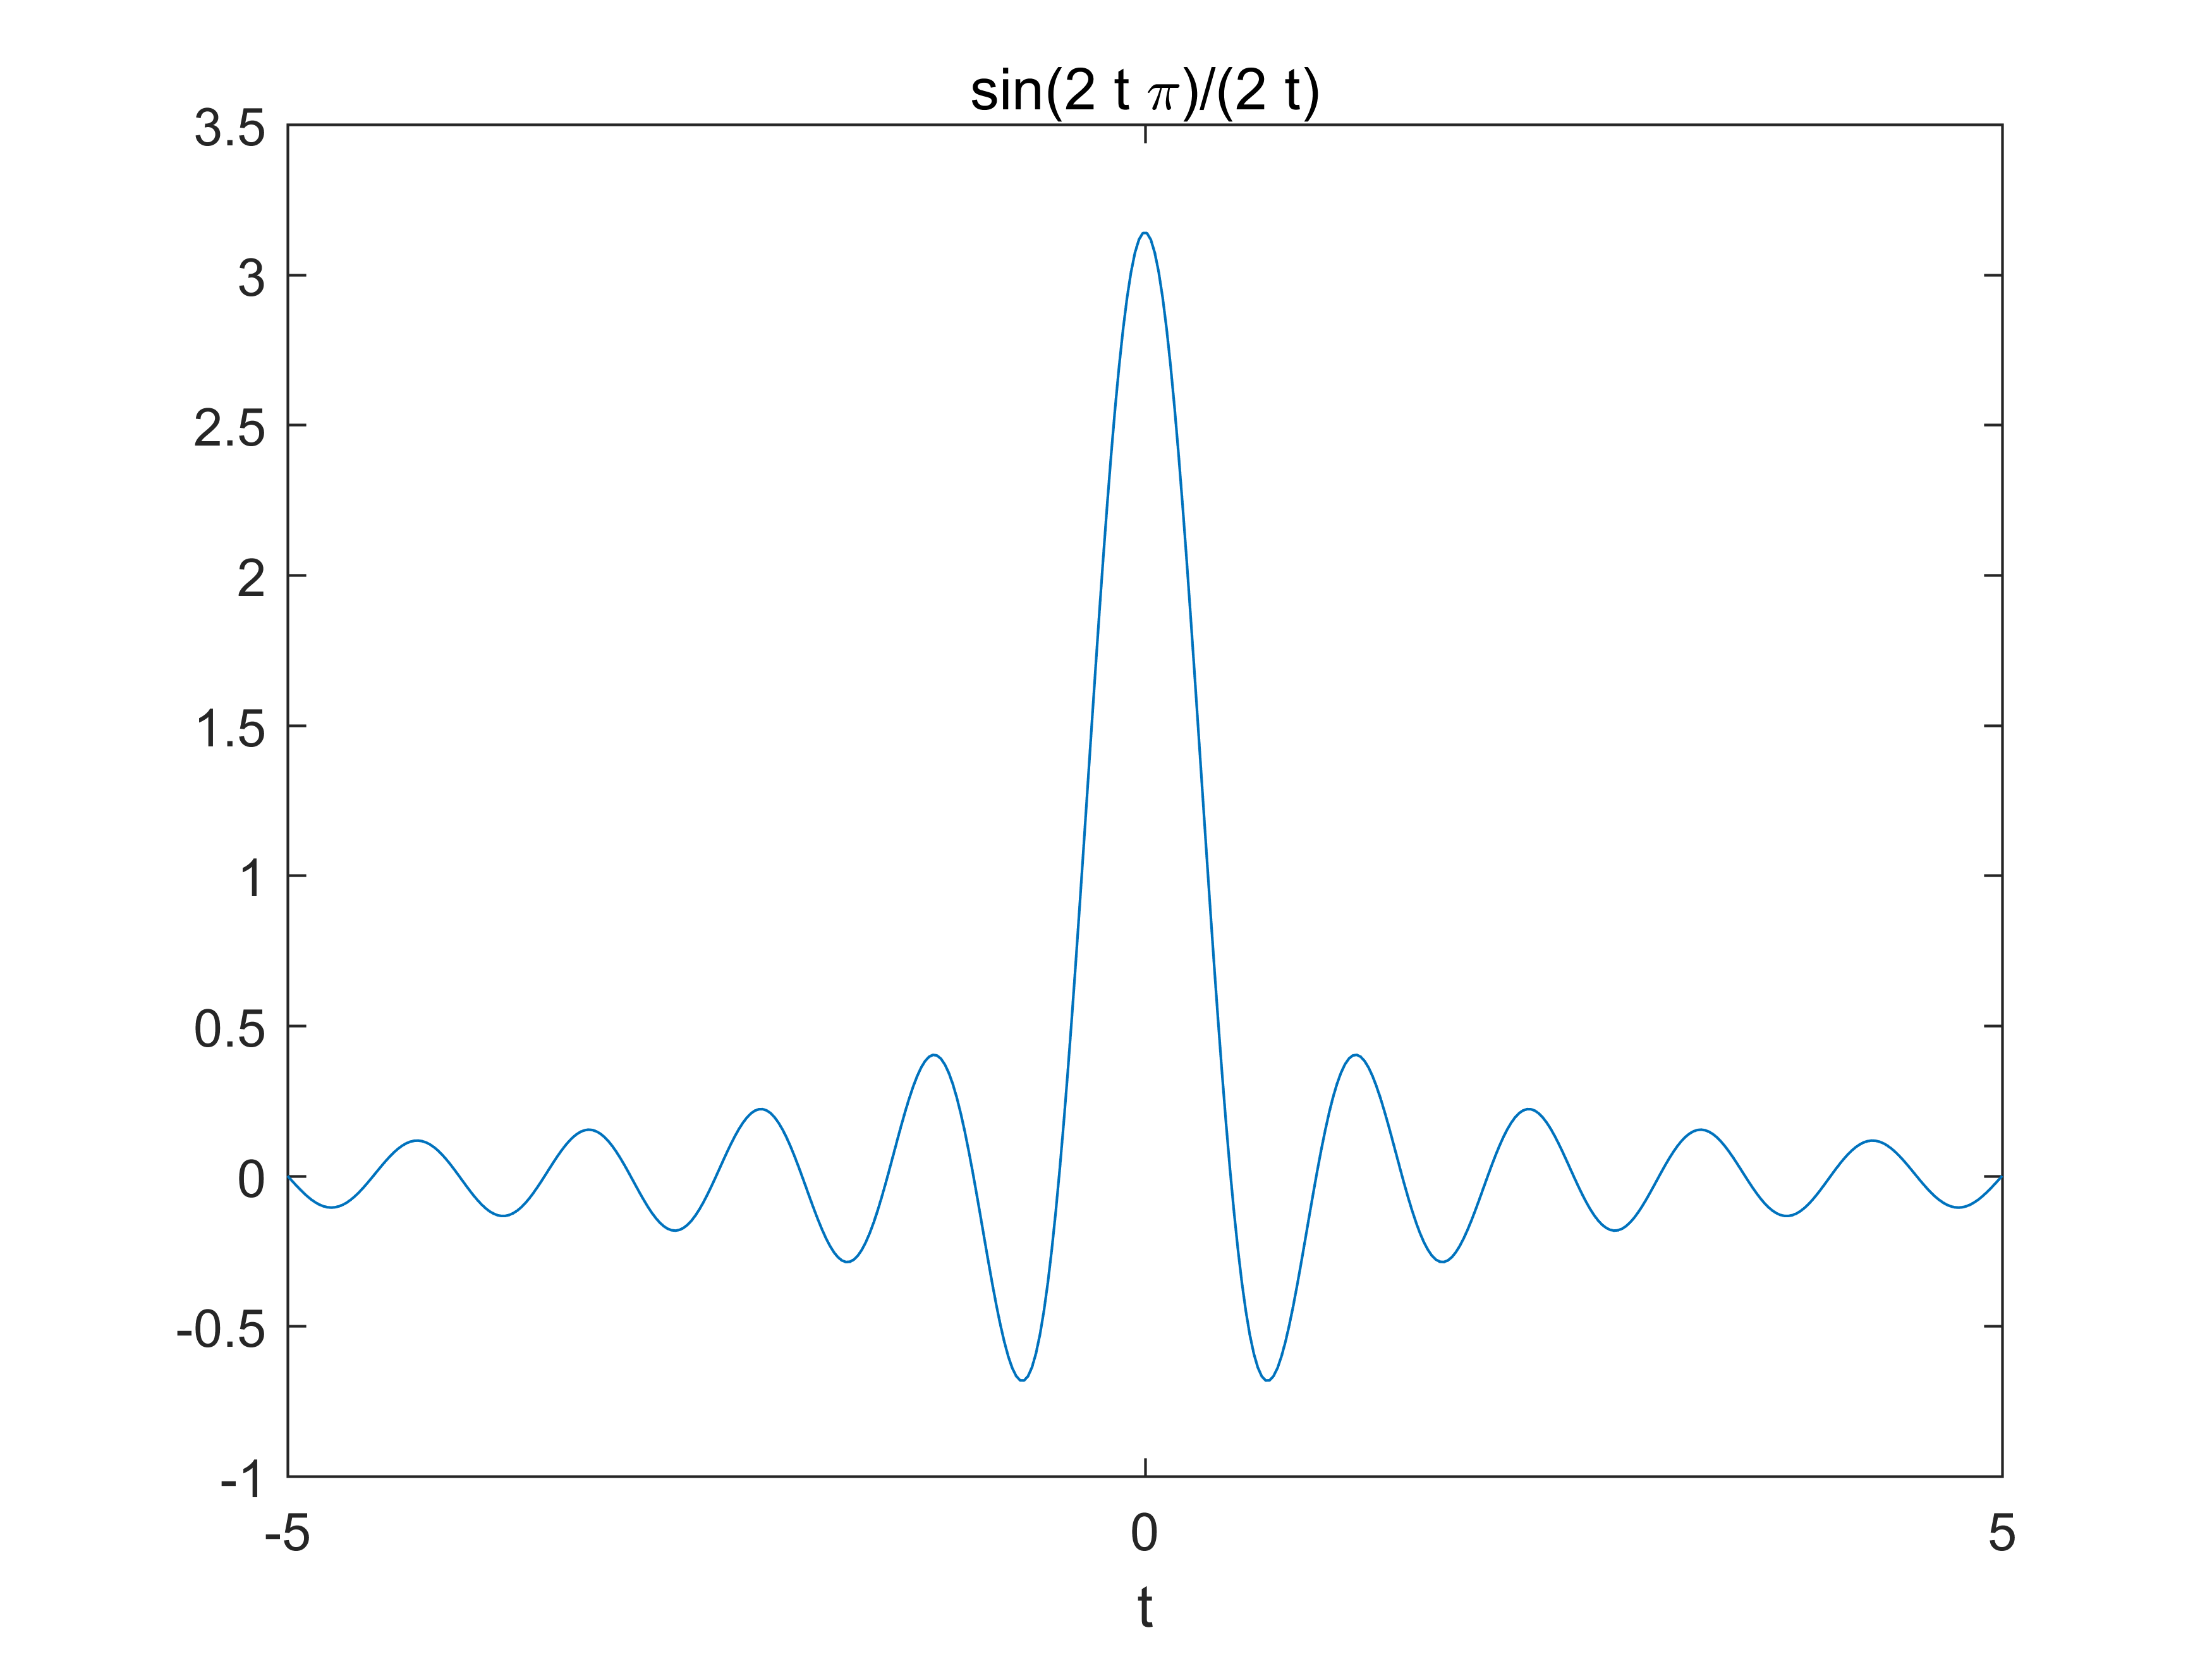
\includegraphics[scale=0.6]{4-1.png}\\
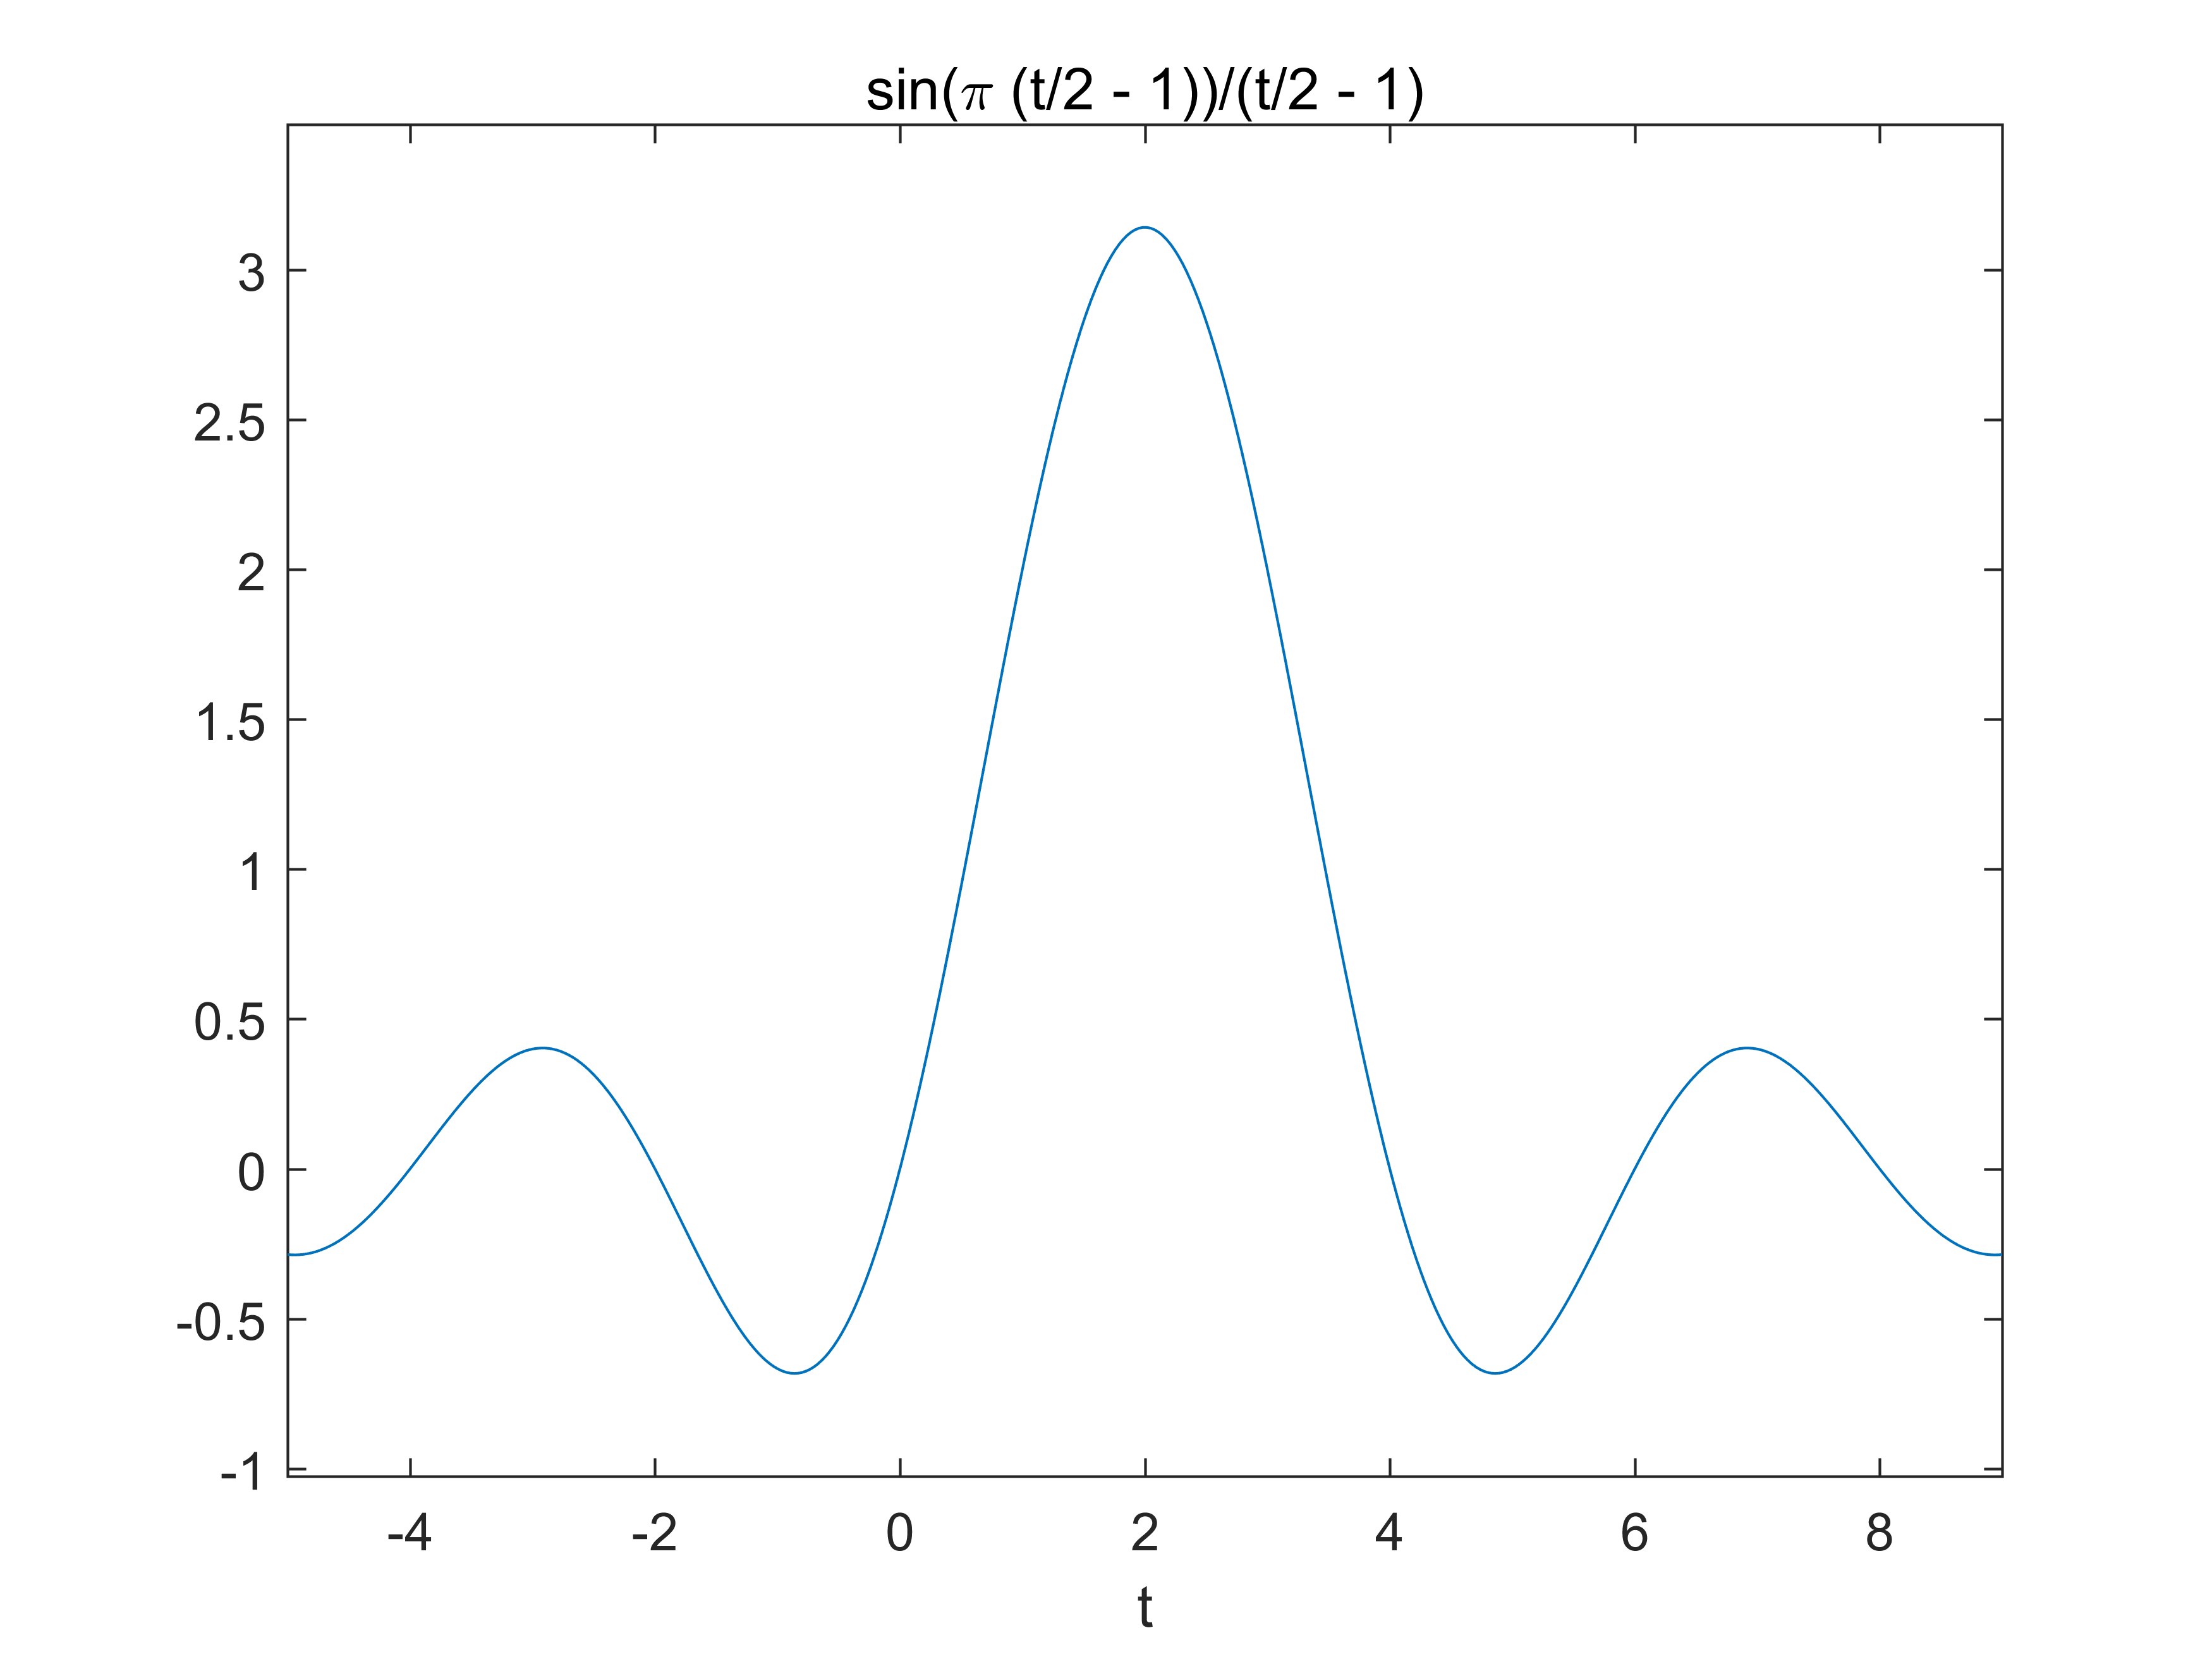
\includegraphics[scale=0.6]{4-2.png}

\end{document}